\documentclass[12pt]{article}
\usepackage[top=1in, bottom=1in, left=.75in, right=.75in]{geometry}
\usepackage{amsmath}


%\usepackage{draftwatermark}
%\SetWatermarkText{draft}
%\SetWatermarkScale{1}
%\SetWatermarkLightness{.9}

%\usepackage[]{enumitem}
\usepackage{enumerate}
\usepackage{fancyhdr}
\usepackage{graphicx, xcolor, setspace, adjustbox}
\usepackage{txfonts}
\usepackage{multicol,coordsys,pgfplots}
\usepackage[scaled=0.86]{helvet}
\renewcommand{\emph}[1]{\textsf{\textbf{#1}}}
\usepackage{anyfontsize}
% \usepackage{times}
% \usepackage[lf]{MinionPro}
\usepackage{tikz,pgfplots}
%\def\degC{{}^\circ{\rm C}}
\def\ra{\rightarrow}
\usetikzlibrary{calc,arrows.meta, shapes, angles, quotes}
\pgfplotsset{compat = newest}
\newcommand{\blank}[1]{\rule{#1}{0.75pt}}

\pgfplotsset{my style/.append style={axis x line=middle, axis y line=
middle, xlabel={$x$}, ylabel={$y$}}}


%\usepackage{draftwatermark}
%\SetWatermarkText{Draft}
%\DraftwatermarkOptions{color={[gray]{.9}}}
%\SetWatermarkScale{1.5}

%axis equal

%yticklabels={,,} , xticklabels={,,}

% \setmainfont{Times}
% \def\sansfont{Lucida Grande Bold}
\parindent 0pt
\parskip 4pt
\pagestyle{fancy}
\fancyfoot[C]{\emph{\thepage}}
\fancyfoot[R]{v2}
\fancyhead[L]{\ifnum \value{page} > 1\relax\emph{Math F251X Calculus I: Final Exam}\fi}
\fancyhead[R]{\ifnum \value{page} > 1\relax\emph{Spring 2024}\fi}
\headheight 15pt
\renewcommand{\headrulewidth}{0pt}
\renewcommand{\footrulewidth}{0pt}
\let\ds\displaystyle
\def\continued{{\emph {Continued....}}}
\def\continuing{{\emph {Problem \arabic{probcount} continued....}}\par\vskip 4pt}


\newcounter{probcount}
\newcounter{subprobcount}
\newcounter{subsubprobcount}
\newcommand{\thesubproblem}{\emph{\alph{subprobcount}.}}
\newcommand{\thesubsubproblem}{\emph{\roman{subsubprobcount}.}}
\def\problem#1{\setcounter{subprobcount}{0}%
\addtocounter{probcount}{1}{\emph{\arabic{probcount}.\hskip 1em(#1)}}\par}
\def\subproblem#1{\par\hangindent=1em\hangafter=0{%
\addtocounter{subprobcount}{1}\thesubproblem\emph{#1}\hskip 1em}}
\def\subsubproblem#1{\par\hangindent=1em\hangafter=0{%
\addtocounter{subsubprobcount}{1}\thesubsubproblem\emph{#1}\hskip 1em}}
\def\probskip{\vskip 10pt}
\def\medprobskip{\vskip 2in}
\def\subprobskip{\vskip 45pt}
\def\bigprobskip{\vskip 4in}


\newenvironment{subproblems}{%
\begin{enumerate}%
\setcounter{enumi}{\value{subprobcount}}%
\renewcommand{\theenumi}{\emph{\alph{enumi}}}}%
{\setcounter{subprobcount}{\value{enumi}}\end{enumerate}}

\newenvironment{subsubproblems}{%
\begin{enumerate}%
\setcounter{enumi}{\value{subsubprobcount}}%
\renewcommand{\theenumi}{\emph{\roman{enumi}}}}%
{\setcounter{subprobcount}{\value{enumi}}\end{enumerate}}


\newcommand{\be}{\begin{enumerate}}
\newcommand{\ee}{\end{enumerate}}


\begin{document}

{\emph{\fontsize{26}{28}\selectfont Spring 2024 \hfill
\hfill Math F251X}}

\begin{center}
{\emph{\fontsize{32}{36}\selectfont Calculus I: Final Exam}}
\end{center}
\vskip 1.cm

\strut\vtop{\halign{\emph#\hskip 0.5em\hfil&#\hbox to 2in{\hrulefill}\cr
\emph{\fontsize{18}{22}\selectfont Name:}&\cr
\noalign{\vskip 10pt}
%\emph{\fontsize{18}{22}\selectfont Student Id:}&\cr
%\noalign{\vskip 10pt}
%\emph{\fontsize{18}{22}\selectfont Calculator Model:}&\cr
}}
\hfill
\vtop{\halign{\emph{\fontsize{18}{22}\selectfont #}\hfil& \emph{\fontsize{18}{22}\selectfont\hskip 0.5ex $\square$ #}\hfil\cr
Section: & 9:15 (Mohamed Nouh)\cr
\noalign{\vskip 4pt}
         & 11:45 (James Gossell)\cr
\noalign{\vskip 4pt}
         & Online (Leah Berman)\cr}}
%
%\vfill


{\fontsize{16}{18}\selectfont\emph{Rules:}}
\begin{itemize}
\item Partial credit will be awarded, but you must {\bf show your work}.

\item You may have a single handwritten $3'' \times 5''$ notecard, both sides.

\item Calculators are \emph{not allowed}. 

\item Place a box around your  \fbox{FINAL ANSWER} to each question where appropriate.

\item Turn off anything that might go beep during the exam.

\item You have two hours to complete the exam.

\end{itemize}


%If you need extra space, you can use the back sides of the pages.
%Please make it obvious  when you have done so.

%Good luck!
%\vfill
\def\emptybox{\hbox to 2em{\vrule height 16pt depth 8pt width 0pt\hfil}}
\def\tline{\noalign{\hrule}}
\centerline{\vbox{\offinterlineskip
{
\bf\sf\fontsize{18pt}{22pt}\selectfont
\hrule
\halign{
\vrule#&\strut\quad\hfil#\hfil\quad&\vrule#&\quad\hfil#\hfil\quad
&\vrule#&\quad\hfil#\hfil\quad&\vrule#\cr
height 3pt&\omit&&\omit&&\omit&\cr
&Problem&&Possible&&Score&\cr\tline
height 3pt&\omit&&\omit&&\omit&\cr
&1&&12&&\emptybox&\cr\tline
&2&&10&&\emptybox&\cr\tline
&3&&10&&\emptybox&\cr\tline
&4&&12&&\emptybox&\cr\tline
&5&&11&&\emptybox&\cr\tline
&6&&10&&\emptybox&\cr\tline
&7&&8&&\emptybox&\cr\tline
&8&&12&&\emptybox&\cr\tline
&9&&11&&\emptybox&\cr\tline 
&10&&4&&\emptybox&\cr\tline 
%&11&&?&&\emptybox&\cr\tline \tline 
&Extra Credit&&(5)&&\emptybox&\cr\tline \hline
&Total&&100&&\emptybox&\cr
}\hrule}}}

\newpage
%\begin{enumerate}
%%%%





%%%%%%%%%%%%%%%%% Compute some integrals
\problem{12 points} Compute the following \emph{integrals}. Give the most general answer, and show your work. Clearly indicate any substitutions you use in such a way that someone else can follow your work.



\begin{subproblems}
	\item  $\displaystyle{ \int \sqrt[5]{x^{3}} + \sqrt{3} - \cos(x)\: dx }$
	\vfill
	\item $\displaystyle \int%_{0}^{2} 
	\frac{x^3}{\sqrt{1+x^4}} \: dx$
	\vfill
	\item $\displaystyle{ \int \frac{2x \ln(x^2 +4)}{ x^2 +4}\: dx  }$
	\vfill
	
%	\vfill

\end{subproblems}

\newpage

%%%%%%%%%%% 


%%%%%% 
%%%%%%%%% Graphical stuff
\problem{10 points} Consider the graph of the function $f(x)$ shown below:
	\vspace{-.5cm}
	\begin{center}
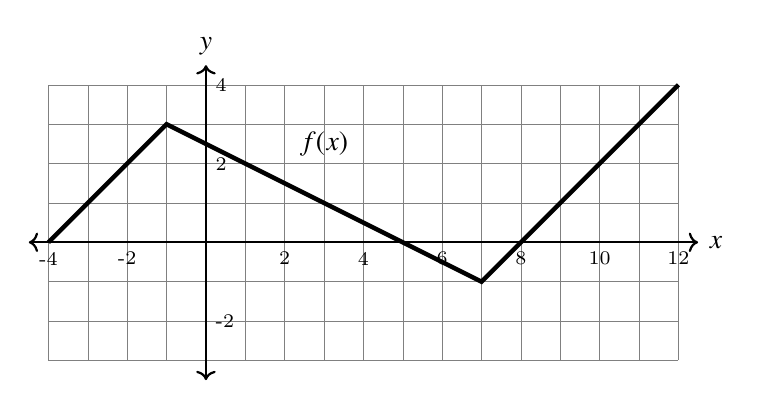
\begin{tikzpicture}[scale = .5]
%cubic
%\begin{axis}[xscale = 1, yscale = 1, thick, my style, xtick={-2,2,4,...,10}, ytick={-1,1,2,3,4},xmin=-5, xmax=10, ymin=-5, ymax=6, minor y tick num=1, minor x tick num=1, 
%mark size=3.0pt, grid = major, ]
%%\addplot[ultra thick, -,domain=-4:-2, samples=100, <-]coordinates {(-4,-2)(-2,2)};
%\addplot[ultra thick, domain=-5:5, samples=100, ,]{sqrt(25-x^2)};
%\addplot[ultra thick, ->,domain=5:9, samples=100]{-1/2*(x-5)};
%\end{axis}

\draw[help lines] (-4, -3) grid (12, 4);
\draw[thick,<->] (-4.5,0) -- (12.5,0) node[right] {$x$};
\draw[thick,<->] (0,-3.5) -- (0,4.5) node[above] {$y$};
%\draw[ultra thick] (5,0) -- (11,-3);
\draw[ultra thick, -] (-4, 0) -- (-1,2+1) -- (7,-2+1) -- (12,4);
%\draw[ultra thick] (5,0) arc (0:180:5);
\foreach \i in { -4,-2,2,4,6,8,10, 12} {\path  (\i,0)node[below, font = \scriptsize] {\i};}
\foreach \i in {-2,2,4} {\path  (0, \i)node[right, font = \scriptsize] {\i};}
\node at (3,2.5) {$f(x)$};
\end{tikzpicture}
\end{center}

\begin{subproblems}
\item Compute $\ds{\int_{1}^{8}f(x) \ dx}$. Show some work or say something about what you computed.

\vfill


\item  Let $\ds{F(t) = \int_{-4}^{t} f(x) \ dx}$. 
\emph{On the interval} $[-4, 12]$, where is $F(t)$ increasing? Where is $F(t)$ decreasing? Write your answers in interval notation.%at what $t$-value does $F(t)$ have an absolute maximum? Where does it have an absolute minumum? 

\smallskip

\begin{itemize}
%\begin{enumerate}[font = \sffamily,label=\textbf{\roman*}.]
	
\item $F(t)$ is \emph{increasing} on the interval \hrulefill %\blank{2cm} %because %\hrulefill. 

\medskip

\item $F(t)$ is \emph{decreasing} on the interval \hrulefill% \blank{2cm} %because %\hrulefill. 

%\end{enumerate}
\end{itemize}

\bigskip

\item Determine $f'(1) = \blank{2cm}$

\bigskip

\item Determine %$\ds\lim_{x \to -1^{-}} f'(x)$ and . (Note that's asking for the limit of the derivative, not the function.) Explain your answer. 
\be[(i)]
\item $\ds\lim_{x \to -1^{-}} f'(x) = \blank{2cm}$
\item $\ds\lim_{x \to -1^{+}} f'(x) = \blank{2cm}$
\item $\ds\lim_{x \to -1} f'(x) = \blank{2cm}$
\ee

%\vfill
\end{subproblems}

\newpage

%%%%%%%%%%%%%%%%% optimization
%\problem{?? points} 
%\begin{minipage}[b]{.6\linewidth}A rectangular storage container with an open top needs to have a volume of $V = 30 \: \textrm{m}^3$. The length $y$ of its base is twice its width $x$. Material for the base costs $ \$ 10$ per $\textrm{m}^{2}$. Material for each of the sides costs $ \$ 5$ per $\textrm{m}^{2}$. 
%\end{minipage}
%%
%\hfill
%%
%\begin{minipage}[b]{.3\linewidth}
%%
%\begin{tikzpicture}[side/.style = { black,thick , fill=gray!50, , fill opacity = .3}, scale = 1.2]
%\pgfmathsetmacro{\cubex}{2} %x width 
%\pgfmathsetmacro{\cubey}{1.2} %z height
%\pgfmathsetmacro{\cubez}{1} %y length
%\draw[side, fill opacity = 1] (0,0,0) -- ++(-\cubex,0,0) -- ++(0,-\cubey,0) -- ++(\cubex,0,0) -- cycle;
%\draw[side, fill opacity = 1] (0,0,0) -- ++(0,0,-\cubez) -- ++(0,-\cubey,0) -- ++(0,0,\cubez) -- cycle;
%
%\draw[side] (-\cubex, -\cubey,-\cubez) -- ++(\cubex,0,0) -- ++(0,\cubey,0) -- ++(-\cubex,0,0) -- cycle;
%\draw[side] (-\cubex, -\cubey,-\cubez) -- ++(0,0,\cubez) -- ++(0,\cubey,0) -- ++(0,0,-\cubez) -- cycle;
%\draw[side,fill=black!80, opacity = .6] (-\cubex, -\cubey,-\cubez) -- ++(\cubex,0,0) -- ++(0,0,\cubez) -- ++(-\cubex,0,0) -- cycle;
%
%\draw[|-|] (-\cubex-.2,0,0)-- node[left]{$z$} +(0, -\cubey, 0);
%\draw[|-|] (0,-\cubey-.2,0)-- node[below]{$y$} +(-\cubex, 0, 0);
%\draw[|-|] (.2,-\cubey-.1,0)-- node[below right]{$x$} +(0, 0, -\cubez);
%%\draw 
%%\path  (-\cubex, -\cubey,-\cubez) node[draw, circle, red]{};
%%\path (0,0,0) node[draw, circle, black]  {};
%%\path (0,-\cubey,0) node[draw, circle, green]  {y};
%%\path (-\cubex,0,0) node[draw, circle, blue]  {x};
%%\path (0,0,-\cubez) node[draw, circle, orange]  {z};
%
%
%\end{tikzpicture}
%
%\end{minipage} 
%
%\begin{subproblems}
%
%\item Write a function, in terms of $x$, that gives the total cost of the container.
%
%\vspace{1.5in}
%
%\item Find the value of $x$ that \emph{minimizes} the cost of the container.
%\vfill
%
%\item %\emph{How much} does the cheapest container cost, and what are its \emph{dimensions}? Answer the question with a sentence.%
%Find the cost of the material for the cheapest container. Write your answer in a sentence.
%
%\vspace{1in} 
%
%\end{subproblems}


%POSSIBLE OTHER PROBLEMS
%
%\#1 


%Find the equation of the tangent line to the curve ${y^{2}=4x^{3}+8x^{2}-12x}$ at the point $(-1,4)$.
\problem{10 points} 
%\begin{minipage}{.5\linewidth}
A portion of the implicitly defined curve
%
\[y^{2} = x^{3}-3x + 3\]
%
%\[y^2 = x^2 \left(\frac{x}{9} + 1\right)\] This has point (-5, 10/3) on it. But it also has a problem at x = 0 because of the self-intersection. Boo.
%$ 3 + xy^{2} = x^{3}$
is shown in the graph. 

\begin{subproblems}
\item Use implicit differentiation to find the \emph{slope} of the tangent line to the curve at the point $(-2, 1)$ (shown as the black dot). Please give an exact answer.%, not a decimal approximation. 
%\end{minipage}

%\begin{minipage}[t]{.6\linewidth}

%\vspace{0pt}


%\item Determine $\ds \frac{dy}{dx}$.

%\vfill
%\vfill
%\end{minipage}
\hfill
\begin{minipage}[t]{.4\linewidth}
\begin{center}
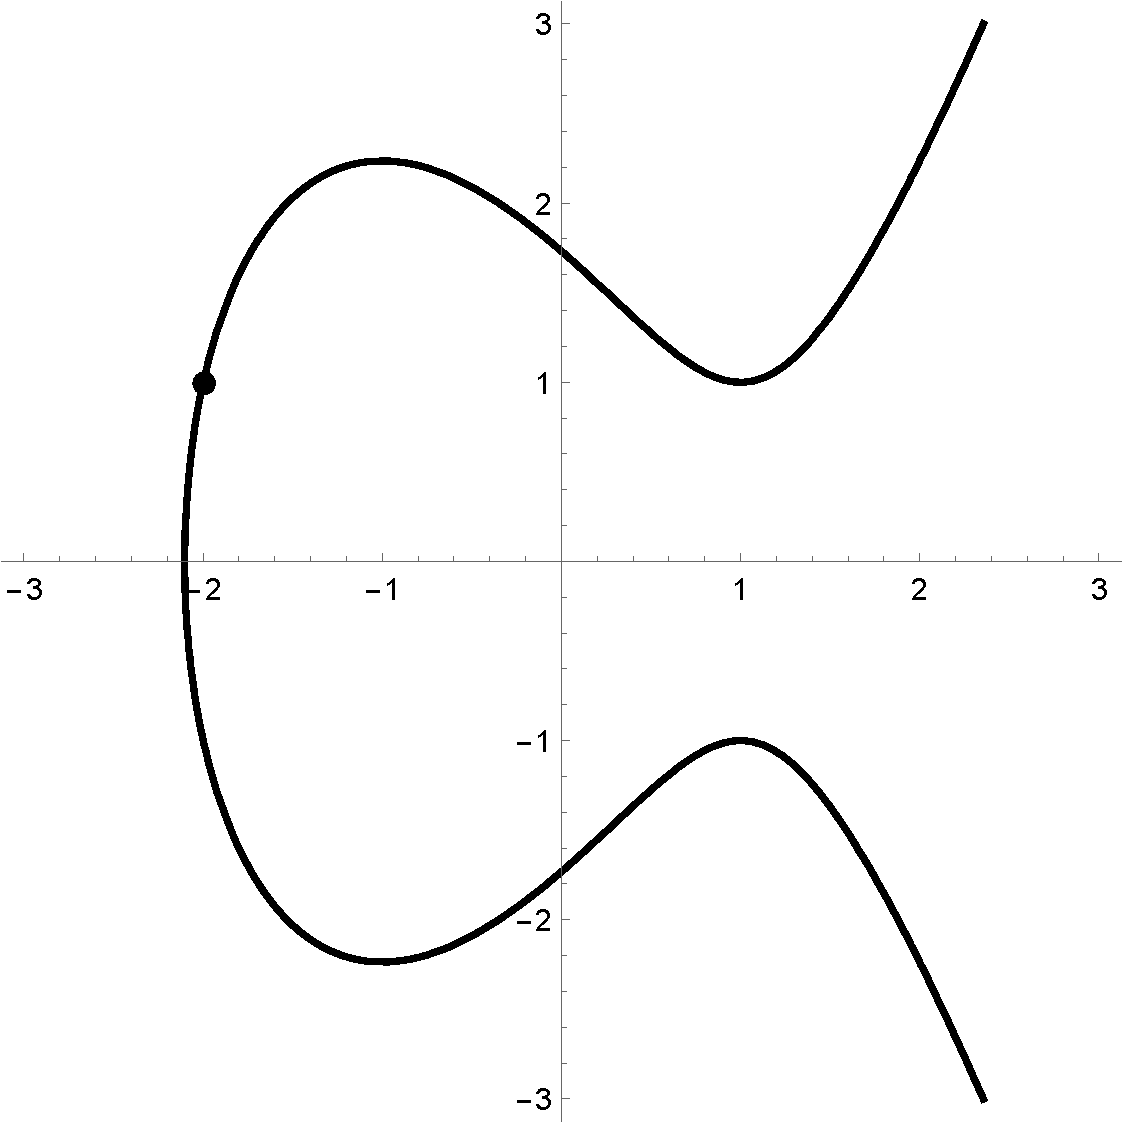
\includegraphics[width=\linewidth]{ImpDifSp24-2.pdf}
\end{center}
\end{minipage}



\item \emph{Write the equation} of the tangent line to the curve at the point $(-2,1)$, which is shown with a black dot on the curve. \emph{Clearly draw and label} the tangent line on the graph. %(Check: does it agree with your equation?)
\vspace{2 cm}

\item Find the coordinates (as ordered pairs) of all points on the curve where the tangent line is horizontal.
\vfill
Coordinates of points: \hrulefill
\end{subproblems}
\newpage

\problem{12 points} A surveillance drone rises from the ground. Its upward velocity is can be modelled by the function \[v(t)=1-e^{-t}\] meters per second at the instant that it is $t$ seconds into its flight.
\begin{subproblems}
\item Compute $v(0)$. Write a complete sentence explaining the meaning of $v(0)$ in the context of the problem. Include units in your answer.
\vfill
\item Compute $\displaystyle \int_0^4 v(t)dt$ and write a sentence to interpret its meaning in the context of the problem. Include units in your answer.
\vfill
\item Find $v'(t)$. Compute $v'(0)$ and write a sentence to interpret its meaning in the context of the problem. Include units in your answer.
\vfill
\end{subproblems}

%\problem{7 points} \begin{minipage}{.7\linewidth}Suppose a rectangular box has two square sides and four sides where the length of the side is two times the width of the side (see diagram).
%
%Suppose the short side of the box is measured to be 10 cm $\pm$ 1 mm (1mm =  1/10 cm), and the volume is computed. Use linearization or differentials to determine the \emph{error} in the measurement of the volume.  Write your answer with a sentence, using correct units.\end{minipage}
%    \hspace{1cm}
%\begin{minipage}{.3\linewidth}
%\begin{tikzpicture}[side/.style = { black,thick , fill=gray!50, , fill opacity = .3}, scale = 1.0]
%\pgfmathsetmacro{\cubex}{2} %x width 
%\pgfmathsetmacro{\cubey}{1} %z height
%\pgfmathsetmacro{\cubez}{1} %y length
%\draw[side, ] (0,0,0) -- ++(-\cubex,0,0) -- ++(0,-\cubey,0) -- ++(\cubex,0,0) -- cycle;
%\draw[side,] (0,0,0) -- ++(0,0,-\cubez) -- ++(0,-\cubey,0) -- ++(0,0,\cubez) -- cycle;
%
%\draw[side] (-\cubex, -\cubey,-\cubez) -- ++(\cubex,0,0) -- ++(0,\cubey,0) -- ++(-\cubex,0,0) -- cycle;
%\draw[side] (-\cubex, -\cubey,-\cubez) -- ++(0,0,\cubez) -- ++(0,\cubey,0) -- ++(0,0,-\cubez) -- cycle;
%\draw[side,%fill=black!80, opacity = .6
%] (-\cubex, -\cubey,-\cubez) -- ++(\cubex,0,0) -- ++(0,0,\cubez) -- ++(-\cubex,0,0) -- cycle;
%
%\draw[|-|] (-\cubex-.2,0,0)-- node[left]{$x$} +(0, -\cubey, 0);
%\draw[|-|] (0,-\cubey-.2,0)-- node[below]{$2x$} +(-\cubex, 0, 0);
%\draw[|-|] (.2,-\cubey-.1,0)-- node[below right]{$x$} +(0, 0, -\cubez);
%%\draw 
%%\path  (-\cubex, -\cubey,-\cubez) node[draw, circle, red]{};
%%\path (0,0,0) node[draw, circle, black]  {};
%%\path (0,-\cubey,0) node[draw, circle, green]  {y};
%%\path (-\cubex,0,0) node[draw, circle, blue]  {x};
%%\path (0,0,-\cubez) node[draw, circle, orange]  {z};
%
%
%\end{tikzpicture}
%\end{minipage}
%
%
%\vfill
%
%\vfill
%
%\vfill

%(ii) Determine the \emph{percent} error in the computation?

\newpage

%%%%%%%%%%%%%%%%%%%% OPTIMIZAION
\problem{11 points} 

We want to answer the following question: which points on the graph of $y = 9 - x^{2}$ are \emph{closest} to the point $(0,4)$?

It is a mathematical fact that to minimize the distance between two points, it is sufficient to minimize the \emph{square} of the distance.
The function 
\[D(x) = (x-0)^{2} + ((9-x^{2}) - 4)^{2} = x^{4} - 9x^{2}+25\]
gives the square of the distance between the point $Q = (0,4)$ and an arbitrary point $P = (x,y) = (x, 9-x^{2})$ on the graph.

Determine the $x$-value(s) which {\bf minimize} $D(x)$ in order to find the point(s) on the graph that are closest to the point (0,4). Use Calculus to justify your answer. 

\hfill 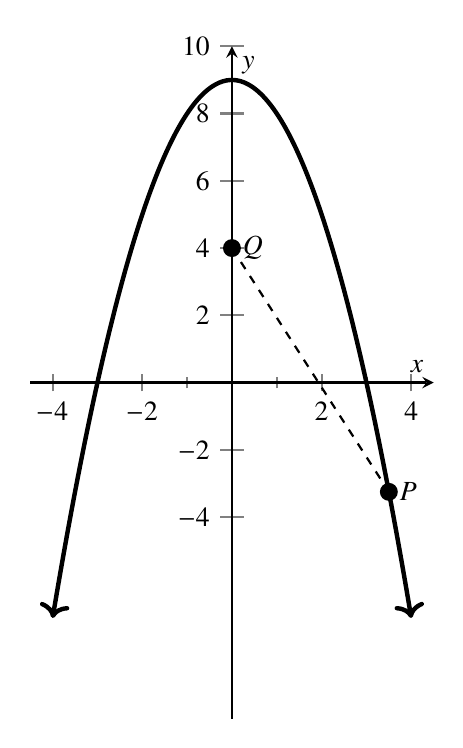
\begin{tikzpicture}
\begin{axis}[xscale=2, yscale = 1.5, thick, my style, xtick={-4, -2,...,5}, ytick={-4,-2,...,10},
xmin=-4.5, xmax=4.5, ymin=-10, ymax=10, minor y tick num=0,tick style = {thick},
        minor x tick num=1, mark size=3.0pt, grid=none, grid style={ thin, black!60}, axis equal image]
% %%asymptote
%\addplot[dashed,<->, ultra thick] coordinates {(5,-4) (5,4)};       
%%%points solid
%\addplot[mark=*,only marks] coordinates {(-4,6)};
%%%points open
%\addplot[mark=*,fill=white,only marks] coordinates {(-2,2)(1,1)(1,-1)(3,-3)};
%%%Curves
%%\addplot[ultra thick, smooth, ->] coordinates {(-5,2)(-4,1)(-3,1.1)(-2.3,3)(-2.1,6.2)};
%\addplot[ultra thick, smooth] coordinates {(-5,-2) (-2,2)};
\addplot[<->,ultra thick, smooth, variable=\x, samples=100, domain=-4:4] plot(\x,9-\x*\x);   
%\addplot[ultra thick, smooth, ->] coordinates {(3,-3)(4, -2.5)(4.5,-1)(4.8, 4)}; 
%\addplot[ultra thick, smooth, ] coordinates {(1,1)(3,1)}; 
%\addplot[ultra thick, smooth, -] (-2,2) parabola  (1,-1);
%\node at (3.5,5){\large{$y$}};
%\draw[fill= black] (0,4) circle (2 pt and 3/2 pt);
\node[draw, circle,fill = black, inner sep = 2pt] (Q) at (0,4){};
\node[draw, circle,fill = black, inner sep = 2pt] (P) at ($(3.5, {9-(3.5)^2})$) {};
%\draw[fill = black (2.5, 9-(2.5)^{2})circle (2 pt and 2 pt) node[right]
\path (P) node[right]{$P$};
\path (Q) node[right]{$Q$};
\draw[dashed] (0,4) -- (P);
\end{axis}
\end{tikzpicture}

\vfill

The closest point(s) is/are : \hrulefill 

(your answer should be (an) ordered pair(s)!)
\newpage

%%%%%%%%%%%%%%%% Related Rates

\problem{10 points} 

A giant spherical snowball is melting. Its volume is decreasing at a rate of $2$ cubic meters per hour. \emph{How fast} is the radius of the snowball decreasing when its radius is $3$ meters? (The volume $V$ of a sphere of radius $r$ is given by $\displaystyle V=\frac{4}{3}\pi r^3$.)

Write your answer in a complete sentence using units.


\newpage


%%%%%%%%%% Interp infinite limit etc.
%\problem{6 points} The population of rabbits in a local park, measured since 2011, can be modeled by the equation 
%\[ P(t) = \frac{10\, 000 e^{t/10}}{480 + 20 e^{t/10}}\]
%where $t$ measures time, in years, since 2011.
%
%\begin{subproblems}
%\item How many rabbits were in the park in 2011? Simplify your answer.
%\vspace{1.5cm}
%
%
%\item \emph{Compute} $\ds \lim_{t \to \infty} P(t)$. Show your work clearly, with correct use of notation. 
%
%\vfill
%
%
%\item  \emph{Write a sentence} that explains the meaning of the limit you just calculated, in terms a person who has not taken calculus can understand. 
%
%\vspace{1.5cm}
%
%\end{subproblems}

%%%%%%%% 
\problem{8 points} Compute the following \emph{limits}. Show your work clearly. Make sure you use \emph{limit notation} where required; an answer that does not use proper notation will not receive full credit. Use = to show things are equal. If you use L'H\^opital's rule, write $\stackrel{H}{=}$ or  $\stackrel{L'H}{=}$ to indicate where you are applying it.

\begin{subproblems}
\item $\ds{\lim_{ x\to \infty} \frac{\ln(5x^4 +6)}{x^4}}$ 
\vfill
%\item $\ds \lim_{x \to \infty} \frac{-8x^3 +5x + 1}{2x^3 +3x - 5 }$
%\vfill
\item $\ds{\lim_{ x\to 1} \frac{\sqrt{2-x}-x}{x-1}}$ 
\vfill
\vspace{.5in}
\end{subproblems}

%\newpage

\problem{12 points} Compute the following \emph{derivatives}. Show your work. You do NOT need to simplify your answer. Your answer should start $f'(x)$, $\frac{df}{dx}$ etc.


\begin{subproblems}

	\item  $\displaystyle{ f(\theta) = \ln ( \csc \theta  + \tan \theta )}$
\vfill
	\item   $\ds g(x)=\frac{\sqrt{4}}{5}+\frac{\sqrt{x}}{3}-\frac{2}{\sqrt{x}}$
\vfill


\item  $\ds h(x)=\frac{e^{4x}}{\cos(x)}$
\vfill


\end{subproblems}


\newpage

%%%%%%%%%%%%%%% curve sketching
\problem{11 points} \emph{Sketch} a graph of a function $h(x)$ that satisfies all of the following properties. 

After drawing the graph:

\begin{itemize}
\item \emph{Label} on the graph the following things, if they exist, by drawing a point on the graph and labeling: any local maximums by writing  \textsf{LOCAL MAX}, local minimums by writing \textsf{LOCAL MIN}, inflection points by writing \textsf{IP} 
\item \emph{Draw} any horizontal and vertical asymptotes with dashed lines and \emph{label} them with their equation.
\item \emph{Mark} any important $x$-values and $y$-values (with numbers) on the $x$- and $y$-axes.
\end{itemize}


\emph{Properties:}
\begin{multicols}{2}
\begin{itemize}
\item The domain of $h(x)$ is $(-\infty, \infty)$
\item $h(0)=0$ and $h(2)=-2$
\item $h'(x) > 0$ on the interval $(-\infty, 0)\cup(2,\infty)$
\item $h'(x) < 0$ on the interval $(0,2)$
\columnbreak
\item $h''(x) > 0$ on the interval $(1, 3)$
\item $h''(x) < 0$ on the interval $(-\infty, 1)\cup(3,\infty)$
\item $\ds \lim_{x \to -\infty} h(x) = -\infty$
\item $\ds \lim_{x \to \infty} h(x) = 0$
\end{itemize}
\end{multicols}


\begin{tikzpicture}
\draw[<->] (-8,0) --  (8,0);
\draw[<->] (0,4) -- (0,-4);
\end{tikzpicture}


\newpage




%%%%%%%%% Interp function
\problem{4 points} The graph of a function $g(x)$ is shown below. %On the same set of axes, sketch the graph of its derivative $g'(x)$.

\begin{center}
 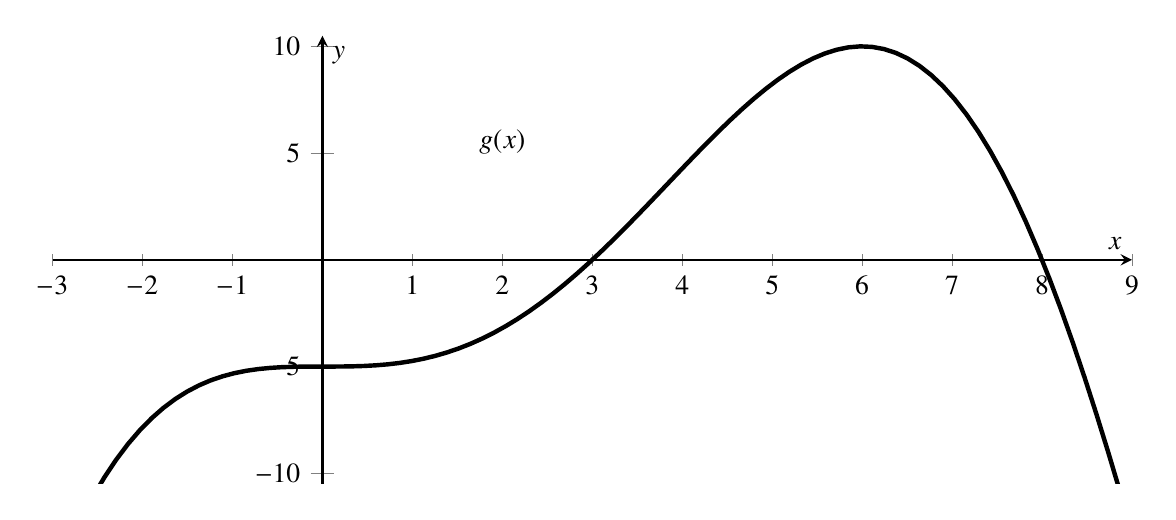
\begin{tikzpicture}
\begin{axis}[scale=1,xscale=2, thick, my style,xmin=-3, xmax=9, ymin=-10.5, ymax=10.5, xtick={-3, ..., 9},
mark size=3.0pt, ]
\addplot[ultra thick, <->,domain=-4:9, samples=100]%{(0.1)*(0.25*x*x*x*x-2*x*x*x+x*x)+4};
{-(5. - 0.299117*x^3 + 0.0335166*x^4 + 0.00218019*x^5 - 0.00023108*x^6)};
%\addplot[ultra thick, <-,domain=-6:0, samples=100]{-x};
\node at (2, 5.5){$g(x)$};
\end{axis}
\end{tikzpicture}
\end{center}

Sketch the graph of its derivative $g'(x)$ on the axes below.

\begin{center}
\begin{tikzpicture}
\begin{axis}[scale=1,xscale=2, thick, my style,xmin=-3, xmax=9, ymin=-10.5, ymax=10.5, ytick=\empty,xtick={-3, ..., 9},
mark size=3.0pt, ]
%\addplot[ultra thick, ->,domain=-4:9, samples=100]{(0.1)*(0.25*x*x*x*x-2*x*x*x+x*x)+4};
%\addplot[]{x};
%\addplot[ultra thick, <-,domain=-6:0, samples=100]{-x};
%\node at (10,2){$g(x)$};
\end{axis}
\end{tikzpicture}\end{center}

\newpage


%\end{enumerate}
%%%%%%%%%%%%%%%%%%%%%%%%%%%

\newpage

%% Extra Credit Newton's Method
\fbox{\emph{Extra Credit}} (5 points) A portion of the graph of the function $f(x)=-3 + x/2 + x^3\:$ is shown below.

	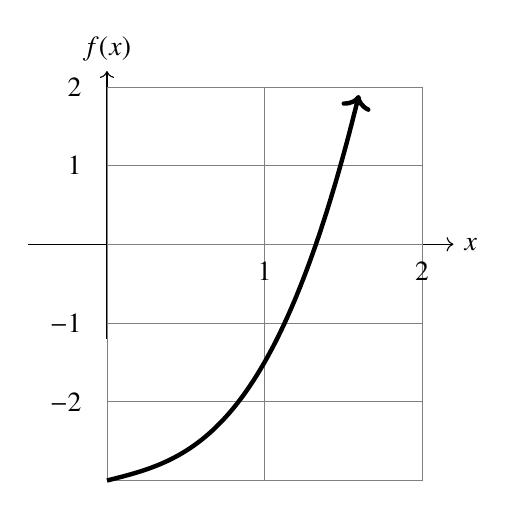
\begin{tikzpicture}[xscale = 2]
\draw[->] (-0.5,0) -- (2.2,0) node[right] {$x$};
\draw[->] (0,-1.2) -- (0,2.2) node[above] {$f(x)$};
\draw[help lines] (-0,-3) grid (2,2);
\foreach \x in {1,2}
\draw (\x,-0.1) node[below] {$\x$};
\foreach \y in {-2,-1,1,2}
\draw (-0.1,\y) node[left] {$\y$};
%\draw[scale=0.5, domain=-3:3, smooth, variable=\x, blue] plot ({\x}, {\x*\x});
	\draw[domain=0:1.6, ->, ultra thick,smooth, variable=\x] plot({\x},{-3 + \x/2 + \x^3});
	\end{tikzpicture}

\begin{enumerate}[a.]%[font = \sffamily,label=\textbf{\alph*}.]
	\item Suppose Newton's method is used to find an approximate solution to
	$f(x)=0$ from an initial guess of $x_1=1$. \emph{Sketch} on the graph how the
	next approximation $x_2$ will be found, \emph{labeling}
	its location on the $x$-axis.
	%\vfill
	\item If your starting guess is $x_1=1$, \emph{compute} $x_2$. 	\vfill
\end{enumerate}

\newpage



\end{document}

%%%%ENDDOCUMENT


